\documentclass{article}%
\usepackage[T1]{fontenc}%
\usepackage[utf8]{inputenc}%
\usepackage{lmodern}%
\usepackage{textcomp}%
\usepackage{lastpage}%
\usepackage{amsmath}%
\usepackage{graphicx}%
%
%
%
\begin{document}%
\normalsize%
\section{linear\_mms}%
\label{sec:linearmms}%
FEA results for the mms function and laplacian:%
\[%
f(x, y) = x + y, l(x, y) = 0%
\]%


\begin{figure}[h!]%
\centering%
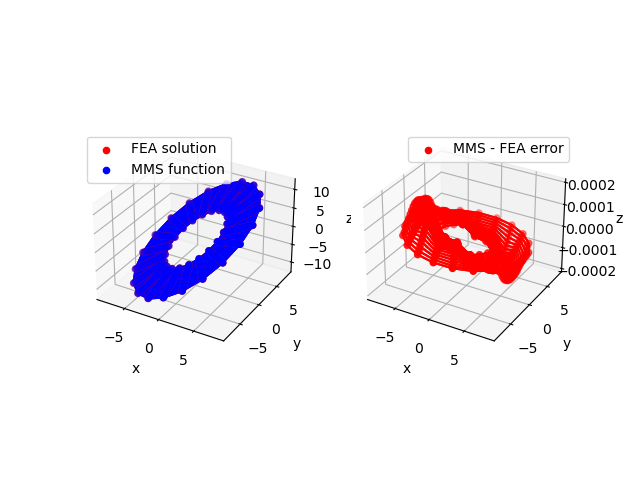
\includegraphics[width=\textwidth]{/Users/zackjensen/school_23/cmp/ZaJeCMP23/MIP_project/fea_grid/test/results/linear_mms.png}%
\end{figure}

%
The $\frac{L2 norm}{n-nodes}$ measure is 4.1306278997434234e-06

%
\newpage%
\section{quadratic\_mms}%
\label{sec:quadraticmms}%
FEA results for the mms function and laplacian:%
\[%
f(x, y) = x^2 + y^2, l(x, y) = 0%
\]%


\begin{figure}[h!]%
\centering%
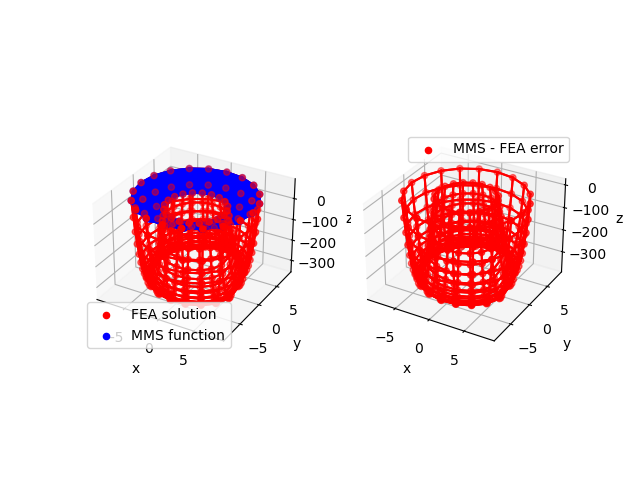
\includegraphics[width=\textwidth]{/Users/zackjensen/school_23/cmp/ZaJeCMP23/MIP_project/fea_grid/test/results/quadratic_mms.png}%
\end{figure}

%
The $\frac{L2 norm}{n-nodes}$ measure is 11.707952741219794

%
\newpage%
\section{cubic\_mms}%
\label{sec:cubicmms}%
FEA results for the mms function and laplacian:%
\[%
f(x, y) = x^3 + y^3, l(x, y) = 6(x + y)%
\]%


\begin{figure}[h!]%
\centering%
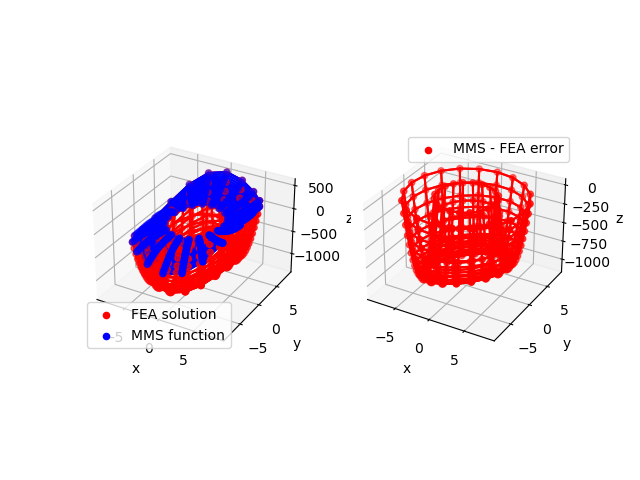
\includegraphics[width=\textwidth]{/Users/zackjensen/school_23/cmp/ZaJeCMP23/MIP_project/fea_grid/test/results/cubic_mms.png}%
\end{figure}

%
The $\frac{L2 norm}{n-nodes}$ measure is 32.98909209465554

%
\newpage%
\end{document}